\documentclass{article}
\usepackage{listings}
\usepackage{graphicx}
\usepackage{float}



\begin{document}

\centerline{\sc \large CS 558: Homework 3}
\vspace{.5pc}
\centerline{Alana Laryssa Seabra A Santos}
\centerline{\it 4/2/2016}
\vspace{1pc}

\section{First problem}

There's really nothing special to point out about my kmeans implementation. Only that I tried to avoid loops the most, and end up calculating lots of matrices representing the distances of the pixels to the potential clusters. The result is below:

\begin{figure}[ht]
\centering
  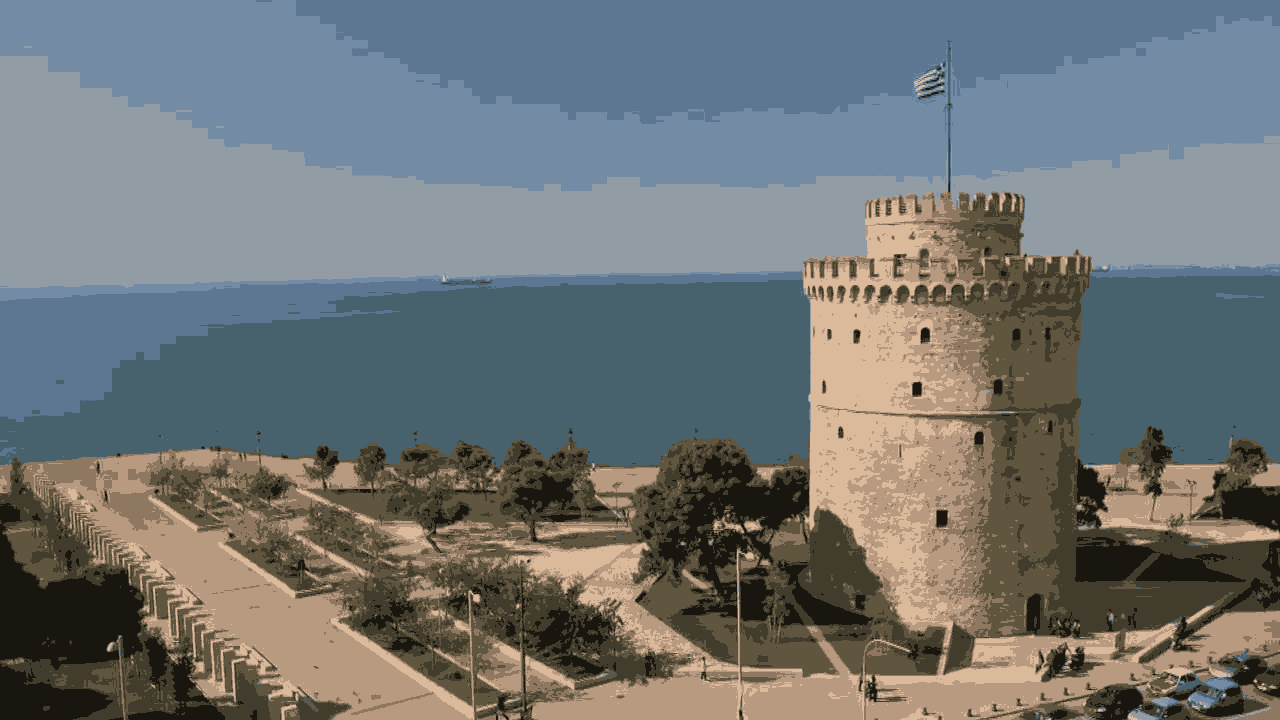
\includegraphics[scale=0.3]{kmeans.png}
\end{figure}

\section{Second problem}

Again the code I wrote was pretty strait forward. The gradients were computed using a 6D vector where the elements were the gradient with sobel filters in x and y over the 3 channels. Then I moved the centroid as proposed, and formed a new 5D vector, consisting of the x and y coordinates of the pixels multiplied by 2 and their 3 channels. This vector is the new image input for kmeans, while the moved centroids are the initial clusters. The results are below.
\\ \\


\begin{figure}[h!]
\centering
  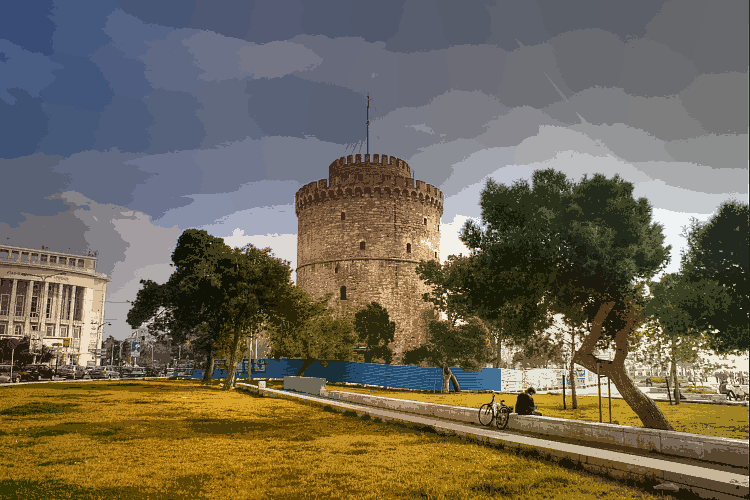
\includegraphics[scale=0.40]{slic1.png}
\end{figure}


\begin{figure}[h!]
\centering
  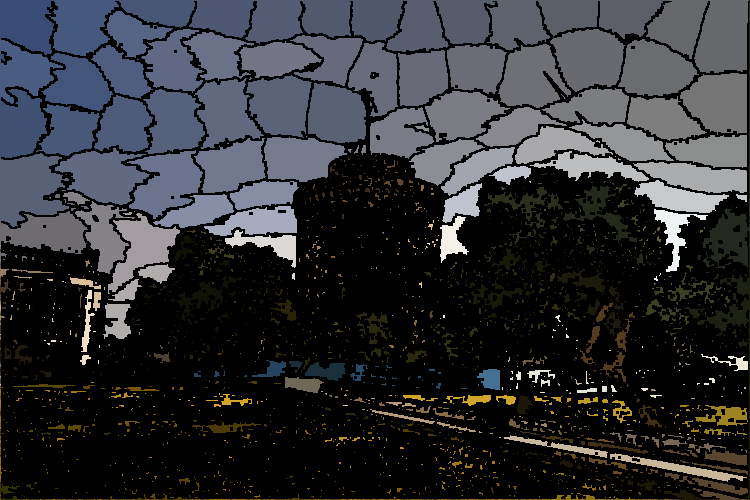
\includegraphics[scale=0.40]{slic2.png}
\end{figure}


\section{Matlab code}
\begin{lstlisting}[language=Matlab]

function im2 = filtering (im, f)
 [s1, s2] = size(f);
 hs1 = (s1-1)/2; hs2 = (s2-1)/2;
 im2 = im; 
 for i = hs1+1 : size(im,1) - hs1
     for j = hs2+1 : size(im,2) - hs2
         im2(i,j) = sum(sum(f.*im(i-hs1:i+hs1, j-hs2:j+hs2)));
     end
 end 
end

function results = kmeansseg(im, k, initial_clusters)
    [s1,s2,s3] = size(im);
    distances = Inf(s1,s2,k);   
    clusters = zeros(k,s3);
    new_clusters = zeros(k,s3);
    
   for i = 1:k
      % only the rgb value
      clusters(i,1:s3) = im(initial_clusters(i,1),initial_clusters(i,2),:);
   end
   
   % main loop
   stop = 0;
   iteration = 0;
   while ~stop   
       % calculate the distances from every pixel to every cluster
       for i = 1:k
           auxdiff = [];
           for d = 1:s3
                auxdiff(:,:,d) = repmat(clusters(i,d),s1,s2);
           end
           
           % ||(pi - ci)||
           distt = im - auxdiff;
           distt = power(distt,2);
           distt = sum(distt,3);
           distt = sqrt(distt);

           distances(:,:,i) = distt;
       end
       
       % status holds which cluster each pixel is in
       [~,status] = min(distances,[],3);
       
       for i = 1:k
            % getting the RGB value of pixels in each cluster
            idx = status == i;
            qtd = sum(idx(:));   
            idxmat = repmat(idx,1,1,s3);
            rgb = im(idxmat);
            rgb = reshape(rgb,qtd,s3);
            new_clusters(i,:) = round(mean(rgb)); % rgb values are integers            
       end      
       
       if abs(norm(new_clusters) - norm(clusters)) < 0.1
           stop = 1;
       end
             
       clusters = new_clusters;
       iteration = iteration + 1;
       
   end   
   
   disp(['total iterations: ' num2str(iteration)])
   results = zeros(size(im));
   for x = 1:s1
       for y = 1:s2
           results(x,y,:) = clusters(status(x,y),:);           
       end
   end
end


function results = slic(im,win)

    [s1,s2,~] = size(im);

    % centroids
    centr = zeros(s1, s2);
    half = round((win+1)/2);

    centr(half,half) = 1;
    for i = half:win:s1
        for j = half:win:s2
            centr(i,j) = 1;
        end
    end
    
    qtd = sum(centr(:));
    
    % gradient magnitude
    Sx = [-1 0 1; -2 0 2; -1 0 1];
    Sy = [1 2 1; 0 0 0; -1 -2 -1];

    gradient(:,:,1) = filtering(im(:,:,1), Sx);
    gradient(:,:,2) = filtering(im(:,:,2), Sx);
    gradient(:,:,3) = filtering(im(:,:,3), Sx);
    gradient(:,:,4) = filtering(im(:,:,1), Sy);
    gradient(:,:,5) = filtering(im(:,:,2), Sy);
    gradient(:,:,6) = filtering(im(:,:,3), Sy);
    
    gradient = power(gradient,2);
    gradient = sum(gradient,3);
    gradient = sqrt(gradient);
       
    centridx = find(centr==1);
    for i = 1:qtd
        [x,y] = ind2sub(size(im),centridx(i));
        window = gradient(x-1:x+1,y-1:y+1);
        [~,ii] = min(window(:));
        [xf,yf] = ind2sub(size(window),ii);
        xf = xf - 2;
        yf = yf - 2;
        centr(x,y) = 0;
        centr(x+xf,y+yf) = 1;
        initial_clusters(i,:) = [x+xf y+yf];
    end
      
    [xx,yy] = meshgrid(1:s1,1:s2);
    xx = xx';
    yy = yy';
    
    input(:,:,1) = xx./2;
    input(:,:,2) = yy./2;
    input(:,:,3:5) = im;  
    
    results = kmeansseg(input,qtd,initial_clusters);      
end

function im2 = adjusttoplot(im)
    [s1,s2,~] = size(im);   
    im2 = im;
   
    for i = 2:s1-1
        for j = 2:s2-1            
            iff(1,:) = im(i-1,j-1,:) == im(i,j,:);
            iff(2,:) = im(i-1,j,:) == im(i,j,:);
            iff(3,:) = im(i-1,j+1,:) == im(i,j,:);
            iff(4,:) = im(i,j-1,:) == im(i,j,:);
            iff(5,:) = im(i,j+1,:) == im(i,j,:);
            iff(6,:) = im(i+1,j-1,:) == im(i,j,:);
            iff(7,:) = im(i+1,j,:) == im(i,j,:);
            iff(8,:) = im(i+1,j+1,:) == im(i,j,:);
            if sum(iff(:)) ~= 24
                im2(i,j,:) = [0 0 0];
            end            
        end
    end

    imshow(im2);
end


clear all; clc; close all;

im1 = imread('cs558s16_hw3/white-tower.png');
im2 = imread('cs558s16_hw3/wt_slic.png');

% im1 = im2double(im1);
% im2 = im2double(im2);

im1 = double(im1);
im2 = double(im2);

% k means segmentation
k = 10;
initial_clusters = rand(k,2);
initial_clusters(:,1) = round(initial_clusters(:,1).*size(im1,1))+1;
initial_clusters(:,2) = round(initial_clusters(:,2).*size(im1,2))+1;
clusters = kmeansseg(im1,k,initial_clusters);
% back to image
clusters = uint8(clusters);
figure;
imshow(clusters);
% imwrite(clusters, 'hw3latex/kmeans.png');

% SLIC
win = 50;
clusters2 = slic(im2,win);
% back to image
clusters2 = uint8(clusters2(:,:,3:5));
figure;
imshow(clusters2);

adjusttoplot(clusters2);
% imwrite(clusters2, 'hw3latex/slic1.png');


\end{lstlisting}

\end{document}


